\documentclass[A4paper]{article}
\usepackage[a4paper, total={7.2in, 10.5in}]{geometry}
\usepackage{tikz}
\usetikzlibrary{calc}
\usepackage{setspace}
\usepackage{graphicx}
\usepackage{amsmath}
\DeclareMathOperator\cis{cis}
\usepackage{pgfplots}
\graphicspath{ {./images/} }
\usepackage{bookmark}
\setcounter{tocdepth}{2}

\hypersetup{
	colorlinks   = true, %Colours links instead of ugly boxes
	urlcolor     = blue, %Colour for external hyperlinks
	linkcolor    = black, %Colour of internal links
	citecolor   = red %Colour of citations
}

\newcommand{\tikzAngleOfLine}{\tikz@AngleOfLine}
\def\tikz@AngleOfLine(#1)(#2)#3{%
	\pgfmathanglebetweenpoints{%
		\pgfpointanchor{#1}{center}}{%
		\pgfpointanchor{#2}{center}}
	\pgfmathsetmacro{#3}{\pgfmathresult}%
}

\begin{document}
	\tableofcontents
	\pagebreak
	\section{Proof}
	\section{Complex numbers}
	\subsection{Forms expressing complex number}
	\begin{tikzpicture}
		\draw[->, thick] (-0.5,0)--(4,0) node[right]{$x$};
		\draw[->, thick] (0,-0.5)--(0,3.5) node[above]{$y$};
		\coordinate (O) at (0,0);
		\coordinate (A) at (3.5,0);
		\coordinate (B) at (3.5,3);
		\draw [dotted] (A) -- (B);
		\draw [->] (O) -- (B);
		\node[below] at (2,0) {a};
		\node [right] at (3.5,1.5) {b};
		\node [above left] at (1.75, 1.5) {r};
		\tikzAngleOfLine(O)(A){\AngleStart}
		\tikzAngleOfLine(O)(B){\AngleEnd}
		\draw[black,<->] (O)+(\AngleStart:0.7cm) arc (\AngleStart:\AngleEnd:0.7cm);
		\node [above right] at (0.65, 0) {$\theta$};
	\end{tikzpicture}
	\subsubsection{Cartesian form}
	$z=a+bi$\\
	$\operatorname{Re}(z) = a$, $\operatorname{Im}(z) = b$\\
	$|z|=\sqrt{a^2+b^2}$
	\subsubsection{Polar form}
	$z=(r,\theta)$\\
	$r=\sqrt{a^2+b^2}$, $\theta = \arg(z)$\\
	$a=r\cos\theta$, $b=r\sin\theta$, $\tan\theta=\dfrac{b}{a}$\\
	$z=r\cos\theta+r\sin\theta i = r(\cos\theta+\sin\theta i)=r\cis \theta$

	\subsubsection{Exponential / Euler form}
	$z=re^{i\theta}$


	\subsection{Calculations}
	\begin{itemize}
		\item $z_1z_2=r_1r_2\cis(\theta1+\theta2)=r_1r_2e^{i((\theta1+\theta2))}$
		\item $\dfrac{z_1}{z_2}=\dfrac{r_1}{r_2}\cis(\theta1-\theta2)=\dfrac{r_1}{r_2}e^{i((\theta1-\theta2))}$
		\item $z^n = r^n\cis(n\theta)=r^ne^{i\theta n}$
		\item $\sqrt[n]{z}=\sqrt[n]{r}\cis(\dfrac{\theta+2k\pi}{n})=\sqrt[n]{r}e^{i\dfrac{\theta+2k\pi}{n}}$ ($k=0,1,2,\dots,n-2,n-1$)
		\item $\sqrt{a+ib}=\pm(\sqrt{\dfrac{|z|+a}{2}}+i\dfrac{b}{|b|}\sqrt{\dfrac{|z|-a}{2}})$
		\item $\arg(z_1z_2)=\arg(z_1)+\arg(z_2)$
		\item $\arg(\dfrac{z_1}{z_2})=\arg(z_1)-\arg(z_2)$
	\end{itemize}
	\pagebreak

	\section{Matrices}
	\subsection{Finding determinants}
	\subsection{Finding inverse matrices}
	$2\times2$ matrices:\\
	$\begin{bmatrix}
		a & b\\c & d
	\end{bmatrix}^{-1}=\dfrac{1}{ad-bc}\begin{bmatrix}
	d & -b\\-c & a
	\end{bmatrix}$ \\ \\
	$3\times3$ matrices:

	\pagebreak
	\section{Further algebra and functions}
	\subsection{Vieta's Law}

	\section{Vectors}
	\subsection{Expressing linear equations}
	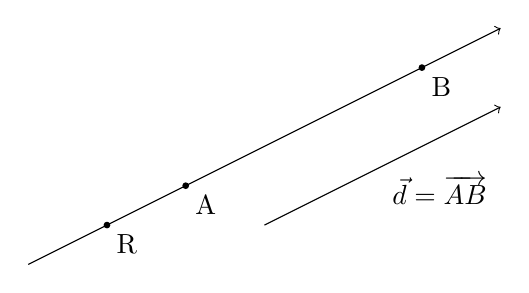
\begin{tikzpicture}
		\draw[->] (0,0) -- (6,3);
		\node[below right] at (1,0.5) {R};
		\filldraw [black] (1,0.5) circle (1pt);
		\node[below right] at (2,1) {A};
		\filldraw [black] (2,1) circle (1pt);
		\node[below right] at (5,2.5) {B};
		\filldraw [black] (5,2.5) circle (1pt);
		\draw[->] (3,0.5) -- (6,2);
		\node[below right] at (4.5,1.25) {$\vec{d}=\overrightarrow{AB}$};
	\end{tikzpicture}

	\subsubsection{Vector form}
	$\vec{r}=\vec{a}+t\vec{d}$ or $(\vec{r}-\vec{a})\times\vec{d}=0$
	\subsubsection{Parametric form}
	$\begin{cases}
		x=x_0+tu\\
		y=y_0+tv\\
		z=z_0+tw
	\end{cases}$
	\subsubsection{Cartesian form}
	$\dfrac{x-x_0}{u}=\dfrac{y-y_0}{v}=\dfrac{z-z_0}{w}=t$

	\subsection{Expressing planes}
	\subsubsection{Vector form}
	\subsubsection{Parametric form}
	$\vec{r}=\vec{a}+t\vec{d}+$
	\subsubsection{Cartesian form}
	When $\vec{n} = \begin{pmatrix}a\\b\\c\end{pmatrix}$: $ax+by+cz=d$

	\subsection{Formulae}
	\subsubsection{Dot and cross product}

	\begin{itemize}
		\item $\vec{a} \cdot \vec{b} = |\vec{a}||\vec{b}|\cos\theta=x_1x_2+y_1y_2+z_1z_2$
		\begin{description}
			\item $\vec{a}\perp\vec{b}$: $\vec{a} \cdot \vec{b} = 0$
			\item $\cos\theta = \dfrac{\vec{a} \cdot \vec{b}}{|\vec{a}||\vec{b}|}$
		\end{description}
		\item $\vec{a} \times \vec{b} = \begin{pmatrix} x_1 \\ x_2 \\ x_3\end{pmatrix} \times \begin{pmatrix} y_1 \\ y_2 \\ y_3\end{pmatrix}=\begin{pmatrix} x_2y_3-x_3y_2 \\ x_3y_1-x_1y_3 \\ x_1y_2-x_2y_1\end{pmatrix}$
		\begin{description}
			\item[Calculating cross product using matrix:] $\begin{vmatrix}
				\vec{i} & \vec{j} & \vec{k} \\
				x_1 & x_2 & x_3 \\
				y_1 & y_2 & y_3
			\end{vmatrix}$
			\item $\vec{a} \times \vec{b} \perp \vec{a}$ and $\vec{a} \times \vec{b} \perp \vec{n}$, so $\vec{a} \times \vec{b} = \vec{n}$
			\item $|\vec{a} \times \vec{b}| = |\vec{a}||\vec{b}|\sin\theta$
			\item $\vec{a}\parallel\vec{b}$: $\vec{a}=\lambda\vec{b}$; $\vec{a} \times \vec{b} = \vec{0}$

		\end{description}
	\end{itemize}
	\subsubsection{Area*}
	Area of triangle $\bigtriangleup ABC$ = $\dfrac{1}{2}|\overrightarrow{AB}\times\overrightarrow{AC}|$\\
	Volume of tetrahedron $ABCD$ = $\dfrac{1}{6}|\overrightarrow{AB}\times\overrightarrow{AC}\cdot\overrightarrow{AD}|$

	\subsection{Questions}
	\subsubsection{Angle between planes}
	\begin{enumerate}
		\item Find the normal of the two planes
		\item Use $\theta = \cos^{-1}\dfrac{\vec{n_1}\cdot\vec{n_2}}{|\vec{n_1}||\vec{n_2}|}$ to find the angle between planes
		\item If $\theta>90$ than the angle is $180-\theta$
	\end{enumerate}
	\subsubsection{Angle between plane and line}
	$\phi = 90-\cos^{-1}\dfrac{\vec{n}\cdot\vec{d}}{|\vec{n}||\vec{d}|}$ or $\phi =\sin^{-1}\dfrac{\vec{n}\cdot\vec{d}}{|\vec{n}||\vec{d}|}$
	\subsubsection{Finding distances between point and line}
	\begin{tikzpicture}
		\coordinate (P) at (4,2);
		\coordinate (T) at (2,1);
		\coordinate (N) at (0.5,4);
		\draw[<-] (0,0) -- (5,2.5);
		\node[below right] at (4,2) {P};
		\filldraw [black] (4,2) circle (1pt);
		\node[below right] at (2,1) {T};
		\draw [dotted] (2,1) -- (0.5, 4);
		\draw [->] (4,2) -- (0.5,4);
		\node[left] at (0.5,4) {N};
		\tikzAngleOfLine(P)(T){\AngleStart}
		\tikzAngleOfLine(P)(N){\AngleEnd}
		\draw[black,<->] (P)+(\AngleStart:0.7cm) arc (\AngleStart:\AngleEnd:0.7cm);
		\node[left] at (3.7,2.05) {$\theta$};
	\end{tikzpicture}\\
	$|\overrightarrow{PT}| = |\overrightarrow{PN}|\cos \theta = \dfrac{\overrightarrow{PN}\cdot\vec{d}}{|\vec{d}|}$\\ $|\overrightarrow{NT}|=\sqrt{|\overrightarrow{PN}|^2-|\overrightarrow{PT}|^2}$
	\subsubsection{Finding distances from point to plane}
	When $P=(x_0,y_0,z_0)$ and the plane has equation $ax+by+cz-d=0$:
	\begin{math}\text{distance}=\dfrac{|ax_0+by_0+cz_0+d|}{\sqrt{a^2+b^2+c^2}}\end{math}
	\subsubsection{Finding distances between lines}
	$\text{distance}=\dfrac{|\overrightarrow{AB}\cdot\vec{n}|}{|\vec{n}|}$


	\pagebreak

	\section{Further algebra and functions}

	\pagebreak

\end{document}